%!TEX root = ../A_Novel_Filtering_Approach_for_Robust_and_Fast_Keypoint_Matching_in_Mobile_Environment.tex

\section{Introduction}

% The very first letter is a 2 line initial drop letter followed
% by the rest of the first word in caps.
% 
% form to use if the first word consists of a single letter:
% \IEEEPARstart{A}{demo} file is ....
% 
% form to use if you need the single drop letter followed by
% normal text (unknown if ever used by IEEE):
% \IEEEPARstart{A}{}demo file is ....
% 
% Some journals put the first two words in caps:
% \IEEEPARstart{T}{his demo} file is ....
% 
% Here we have the typical use of a "T" for an initial drop letter
% and "HIS" in caps to complete the first word.

% \hfill mds
 
% \hfill December 27, 2012

% \subsection{Subsection Heading Here}
% Subsection text here.

% % needed in second column of first page if using \IEEEpubid
% %\IEEEpubidadjcol

% \subsubsection{Subsubsection Heading Here}
% Subsubsection text here.

\IEEEPARstart{I}{mage} matching is a fundamental problem in a variety of computer vision applications, including simultaneous localization and mapping\cite{chang_p-slam:_2007,davison_monoslam:_2007}, object recognition\cite{nister_scalable_2006}, panorama stitching\cite{brown_recognising_2003,wagner_real-time_2010}, augmented reality\cite{klein_parallel_2007,wagner_multiple_2009}, and visual odometry\cite{cheng_visual_2006,nister_visual_2004}. To enhance the image matching quality in various environments, many related techniques have been proposed, such as keypoint-based local matching, histogram-based global matching\cite{le_improving_2013,goncalves_hairis:_2011}, color-based matching\cite{mehtre_color_1995,kankanhalli_cluster-based_1996}, and template-based matching\cite{korman_fast-match:_2013}, etc. Among them, keypoint detection and matching has created great interest since it can provide relatively high matching quality against severe occlusion and do not require segmentation for regions of interest. Also, recent work has concentrated on making invariant to image transformation with low computing power\cite{carrera_robust_2007,mikolajczyk_performance_2005}.


%이미지 매칭 기술은 simultaneous localization and mapping\cite{chang_p-slam:_2007,davison_monoslam:_2007}, object recognition\cite{nister_scalable_2006}, panorama stitching\cite{brown_recognising_2003,wagner_real-time_2010}, augmented reality\cite{klein_parallel_2007,wagner_multiple_2009-1}, visual odometry\cite{cheng_visual_2006,nister_visual_2004} 등 다양한 컴퓨터 비전 연구 분야에서 중요한 기술이다. 이를 해결하기 위하여 Keypoint 기반의 local 매칭 방법\cite{nister_visual_2004,taylor_robust_2009}, histogram 기반의 global 매칭 방법, supervised feature learning, unsupervised feature clustering 방법 등의 연구들이 수행되고 있다. 이 중 영상에서 특징점(interest point or keypoint) 기반의 local 매칭 방법은 영상의 부분 인식에 강인하고, 조명이나 회전 등의 변화에 강인하기 때문에 다양한 이미지 매칭 응용에 활용되고 있다. 

The overall flowchart of keypoint matching and recognition is shown in Fig. \ref{fig:on_offline_process}. These procedure can be divided into two main phases: offline (training) and online (testing) procedure. Offline learning is prerequisite to online matching process. In offline learning phase, a set of reference images to be recognized is analyzed and stored as as types of descriptors in a database. In online learning phase, a newly captured image is analyzed and compared with the reference images in the database to find a nearest reference image. In each phase, common procedures for matching are keypoint detection, description, and matching. To analyze training images, at first, keypoints are detected from the images. Then, from those keypoints, local textures are analyzed and described. In this procedure, to provide robustness against rotation, scale, perspective transform, descriptors are constructed. Then, to be used in online phase, efficient matching structures, as databases, are constructed, such as partitioning trees\cite{arya_optimal_1998,beis_shape_1997,muja_fast_2012}, hashing\cite{salakhutdinov_semantic_2009,gionis_similarity_1999,lv_multi-probe_2007}. In the online matching phase, the database is used to find the most similar corresponding keypoints pair with a given query image. To find the most similar keypoint pairs, with given a query image, keypoints are detected, detected keypoints are described about local texture, and compared with the preconstructed database.

% 이러한 특징점 기반의 local 매칭 방법은, 일반적으로 그림 \ref{fig:on_offline_process}에서 보는 것과 같이 동작한다. 사전에 오프라인 학습 단계에서 미리 학습 영상을 분석하여 데이터베이스를 생성하고, 이를 이용하여 온라인 인식 단계에서 입력된 영상을 데이터베이스와 비교하여 가장 근접한 결과를 검색한다. 이 때 각 단계는, detection, description, matching의 세 가지 단계를 통하여 수행된다. 먼저, 인식의 대상이 되는 train object(reference object)를 분석하여 keypoint database 를 만들게 된다. 이를 위하여 train object image 에서 검출이 잘 되는 점들을 detect 한다. 이렇게 검출된 특징점들에서 local texture 특징을 이용하여 descriptor를 생성한다. 이 단계에서는 rotation, scale, perspective transform 등 다양한 변환에 강인하게 매칭이 수행될 수 있도록 descriptor를 계산한다. 이렇게 계산된 descriptor 집합을 online matching 과정에서 효율적으로 matching이 이루어질 수 있도록 tree나 hashing 과 같은 efficient matching structure 를 만들어 database로 저장한다. 이후 이렇게 만들어진 database를 이용하여 online matching 과정에서는 입력된 query 영상에서 corresponding keypoint pair를 찾게 된다. 이를 위하여 입력된 query 영상에서 특징점을 검출하고, 검출된 특징점의 descriptor를 생성하여 database에 저장된 descriptor와 가장 유사한 특징점을 계산한다. 

\begin{figure}[hb!]
\centering
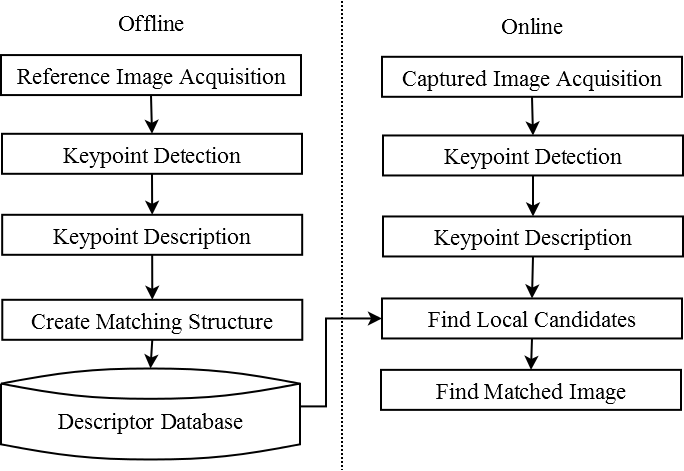
\includegraphics[width=1.0\columnwidth]{1_intro/process}
\caption{Overall process of conventional keypoint-based matching}
\label{fig:on_offline_process}
\end{figure}

Conventional keypoint matching methods stores almost every keypoints which are detected by keypoint detection process. Keypoint detection processes are designed to extract repeatable keypoints and robust against arbitrary image transformation. Then, detected keypoints are independent to the follow matching procedures, and do not reflect quality of descriptors. Therefore, as seen Fig.  some keypoints are not distinguishable, and they tend to cause inter-keypoint confusion and miss matching. \texttt{bad keypoint 이미지 추가} Also, those detected keypoints are stored in database and are compared with keypoints in query images in every frame while matching. Then, it decreases the speed of matching. To overcome these problem, in offline learning procedure, detected keypoints are evaluated with respect to proposed matching quality criteria and filtered by the goodness score. With this filtering method, only a small subset of keypoints is stored in the database. Accordingly, it provides more improved matching performance with faster matching speed.

\begin{figure}[ht!]
\centering
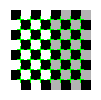
\includegraphics[width=0.5\columnwidth]{1_intro/checkerboard}
\caption{Example of high repeatable but poor distinguishable keypoints. Conventional keypoint matching systems do not consider the discriminability of keypoints, so these keypoints usually stored and negatively affected matching.}
\label{fig:example_of_bad_features}
\end{figure}

%본 논문에서는 database에 저장되는 keypoint들을 평가하여 matching 성능이 높은 점들만 filtering 하여 저장함으로써 matching 성능을 향상시키고 빠른 인식 성능을 제공하는 방법을 제안한다. 기존의 특징점 매칭 방법에서는 일반적으로 keypoint detection process 에서 geometraical 특성에 의하여 저장하고자 하는 특징점들을 filter 하였다. 하지만, 특징점 검출 단계는 영상 변환에도 반복적으로 강인하게 특징점이 검출되는 것을 목표로 설계되었다. 따라서 이렇게 검출된 특징점은 이후의 매칭 단계와는 독립적인 연산이 수행되고, 이에 따라 매칭 퀄리티를 보장할 수 없는 문제가 있다. 이에 따라, 특정 특징점들은 distinguishability가 떨어지는 점들이 학습되는 경우가 많고, 이러한 점들은 miss matching 을 유발하여 인식의 정확도를 떨어뜨리게 된다. (bad keypoint 이미지 추가) 또한, 이러한 점들이 포함된 database는 비교 대상이 되는 특징점의 개수가 증가되므로 인식의 속도 또한 저하시키게 된다.  본 논문에서는 이러한 문제점을 극복하기 위하여 오프라인 학습 단계에서 검출된 특징점의 매칭 성능을 평가하고, 이 평가에 의하여 특징점을 필터링하는 기법을 제안한다. 이를 통하여 매칭 품질이 높은 특징점 만을 저장하고 비교함으로써, 강인한 인식 성능을 제공하면서도 인식의 속도를 향상시킬 수 있는 방법을 제안한다.

Especially, in recent years, mobile computing devices have been widely deployed to customers in recent years, the interest of image matching on mobile devices is increasing. However, mobile devices still have insufficient computing power and limited memory compared to desktop or laptop, then there is an urgent need of effective processing methods for image matching. However, conventional keypoint matching approaches stored redundant keypoints into database, and these redundant keypoints may compared in every frame. So, matching speed will be decreased and this causes problem in the mobile computing devices. So, the proposed method does not store redundant keypoints in the database, it reduces the number of comparisons while matching is done and increase matching speed even in the mobile computing environment.
 
% 이후의 논문은 다음과 같이 구성된다. 먼저 2장에서는 기존의 특징점 기반 매칭 연구들을 정리하고, 이러한 연구 중 기존의 특징점 필터 방법을 설명한다. 3장에서는 제안하는 keypoint score function을 정의하고, 이를 ground truth와 비교하여 유사도를 보여준다. 그리고 이렇게 측정된, 매칭에 유리한 특징점과 그렇지 않은 특징점을 영상 패치로 비교하여 어떤 특징점들이 매칭에 유리한지 설명한다. 이후 4장에서는 다양한 환경에서 실험을 수행하고, 제안하는 방법과 기존의 일반적인 database 방식의 속도 및 인식율, 특징점의 매치 정확도를 비교한다. 이후 5장에서 본론을 정리한다.

This paper is structured as follows: In Section 2, we discuss literature on interesting point detection and matching systems, as well as conventional keypoint filtering algorithms. Section 3 defines the proposed keypoint score function, and we validated the function with matching ground truth data. Then, we compared image patches between match-friendly keypoints and other keypoints set. In Section 4, we executed experiments to prove the proposed keypoint filtering method in various dataset and algorithms and compared over several evaluation metrics. Finally, Section 5 presents the conclusion.

% 기존의 특징점 매칭 방법에서는 특징점 검출 단계에서 검출된 모든 특징점들을 대상으로 레퍼런스 영상을 학습하였다. 하지만, 특징점 검출 단계에서는, 해당 점의 geometrical 특징에 의하여 특징점을 검출하고, 이렇게 검출된 특징점이 반복적으로 검출되는 것을 목표로 한다. 따라서 이렇게 검출된 특징점은 이후의 매칭 단계와는 독립적인 연산이 수행되고, 이에 따라 매칭 퀄리티를 보장할 수 없는 문제가 있다. 본 논문에서는 이러한 문제점을 극복하기 위하여 오프라인 학습 단계에서 검출된 특징점을 평가하고, 이 평가에 의하여 특징점을 필터링하는 기법을 제안한다. 이를 통하여 매칭 품질이 높은 특징점 만을 저장하고 비교함으로써, 강인한 인식 성능을 제공하면서도 인식의 속도를 향상시킬 수 있는 방법을 제안한다.


